\documentclass[12pt,A4paper]{article}
\usepackage[left=1.0in,top=1.0in,bottom=1.0in,right=1.0in]{geometry}
\usepackage{blindtext}
\usepackage{sectsty}
\usepackage{blindtext}
\usepackage{graphicx}
\usepackage{subfig}
\usepackage{listings}
\usepackage{color}
\usepackage[utf8]{inputenc}
\usepackage{amsmath}
\usepackage[english]{babel}
\sectionfont{\fontsize{12}{15}\selectfont}
\subsectionfont{\fontsize{10}{15}\selectfont}
\graphicspath{ {./Figures/} }
\makeatletter
\renewcommand{\@seccntformat}[1]{%
	\ifcsname prefix@#1\endcsname
	\csname prefix@#1\endcsname
	\else
	\csname the#1\endcsname\quad
	\fi}
\addto\captionsenglish{
\renewcommand{\contentsname}
	{Table of Contents}
}
% define \prefix@section
\newcommand\prefix@section{}
\newcommand{\prefix@subsection}{}
\newcommand{\prefix@subsubsection}{}
\renewcommand{\thesubsection}{\arabic{subsection}}
\makeatother
\definecolor{dkgreen}{rgb}{0,0.6,0}
\definecolor{gray}{rgb}{0.5,0.5,0.5}
\definecolor{mauve}{rgb}{0.58,0,0.82}

\lstset{frame=tb,
	language=Matlab,
	aboveskip=3mm,
	belowskip=3mm,
	showstringspaces=false,
	columns=flexible,
	basicstyle={\small\ttfamily},
	numbers=none,
	numberstyle=\tiny\color{gray},
	keywordstyle=\color{blue},
	commentstyle=\color{dkgreen},
	stringstyle=\color{mauve},
	breaklines=true,
	breakatwhitespace=true,
	tabsize=1
}

\begin{document}
	\thispagestyle{empty}
	\begin{center}
		\Huge
		Aer E 261: Final Project \\
		Iowa State University \\
		Jr. JPL \\
		Surveyanator \\
		\vspace{0.25 in}
		
		
		\begin{figure}[!h]
			\centering
			\vspace{0.5 in}
			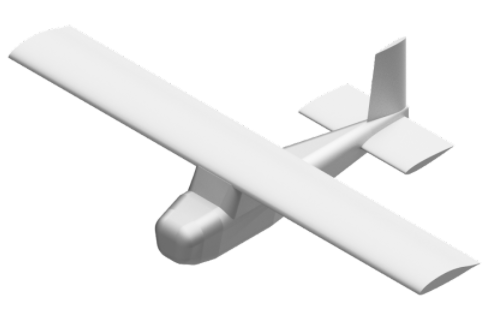
\includegraphics[width=1\textwidth]{IsoCad.png}
			\label{fig:f1}
			\caption{The Surveyanator CAD Model}
		\end{figure}
		\vspace*{\fill}
		\large
		Nicole Buhr, Jeremy Koger, Ellie Mittauer, Justin Pullman, \& Blake Schulte \\
		\vspace{0.25 in}
		Undergraduates in the Department of Aerospace Engineering \\
		Fall 2021 \\
		10 Dec 2021 
		\clearpage
	\end{center}

	\pagenumbering{roman}
	
	\setcounter{page}{2}
	
	\tableofcontents

	\renewcommand\listfigurename{List of Illustrations}
	\listoffigures

	\clearpage
	\pagenumbering{arabic}
	\section{Introduction}
	\section{Requirements}
	\section{Methodology}
	\begin{equation} \label{eq1} 
		M = \frac{V_\infty }{a_\infty} \\ 
	\end{equation}
	\hrule
	\vspace{0.1 in}
	\begin{equation}
		a_\infty = \sqrt{\gamma R T_\infty} \\
	\end{equation}
	\hrule
	\vspace{0.1 in}
	\begin{equation}
		Re = \frac{\rho_\infty v_\infty c}{\mu_\infty} \\
	\end{equation}
	\hrule
	\vspace{0.1 in}
	\begin{equation}
		s = b * c \\
	\end{equation}
	\hrule
	\vspace{0.1 in}
	\begin{equation}
		AR = \frac{b^2}{s} \\
	\end{equation}
	\hrule
	\vspace{0.1 in}
	\begin{equation}
		k = \frac{1}{\pi e_o AR} \\
	\end{equation}
	\hrule
	\vspace{0.1 in}
	\begin{equation}
		a_{3D} = \frac{a_o}{1 + \frac{57.3 a_o}{\pi e AR}} \\
	\end{equation}
	\hrule
	\vspace{0.1 in}
	\begin{equation}
		W_{battery} = \frac{E_{battery}}{E_{density}} *9.81 \\
	\end{equation}
	\hrule
	\vspace{0.1 in}
	\begin{equation}
		C_L = \frac{W_{total}}{\frac{1}{2} \rho  v_\infty^2  s} \\
	\end{equation}
	\hrule
	\vspace{0.1 in}
	\begin{equation}
		\alpha_{3D\_SLF} = \frac{C_L}{a_{3D}}+\alpha_{L=0} \\
	\end{equation}
	\hrule
	\vspace{0.1 in}
	\begin{equation}
		(\frac{C_L}{C_D})_{max} = \sqrt{\frac{1}{4 K C_{D o}}} \\
	\end{equation}
	\hrule
	\vspace{0.1 in}
	\begin{equation}
		(\frac{{C_L}^{1/3}}{C_D})_{max} = \frac{1}{4} (\frac{3}{K C_{D_o}^{1/3}})^{\frac{3}{4}} \\
	\end{equation}
	\hrule
	\vspace{0.1 in}
	\begin{equation}
		Endurance = (\frac{E_{battery} n_{prop} n_{motor} \sqrt{\rho s}}{\sqrt{2} W_{total}^{1.5}} (\frac{{C_L}^{1/3}}{C_D})_{max}) \div 60 \\
	\end{equation}
	\hrule
	\vspace{0.1 in}
	\section{Results}
	\section{Discussion}
	\section{Conclusion}

	\section{References}
	“How to Change a Flat Tire.” Bridgestone Tires, 29 Nov. 2021, https://www.bridgestonetire.com/learn/maintenance/how-to-change-a-flat-tire/.\\ \\
	“How to Change a Tire.” The Home Depot, https://www.homedepot.com/c/ah/how-to-change-a-tire/9ba683603be9fa5395fab908e21cabb.\\ \\
	“How to Change a Tire.” WikiHow, WikiHow, https://www.wikihow.com/Change-a-Tire.\\
	
	
	\section{Code}
	\begin{center}
	Link to Inputs Document: https://docs.google.com/spreadsheets/d/1mX9oFI3Zd5SyJR2twwYRWJ417U7gUv60qco82aeOLdE/\\edit?usp=sharing \\
	\end{center}
	\begin{lstlisting}
		clear,clc,clf
		%AerE 261
		%Jr.JPL Blake, Ellie, Jeremy, Justin, Nicole
		%Surveyanator
		%scaling factor 0.28:1 to the bonanza
		%based of Beechcraft Bonanza and Cessna 172
		
		
		inputs = GetGoogleSpreadsheet('1mX9oFI3Zd5SyJR2twwYRWJ417U7gUv60qco82aeOLdE');
		inputs = str2double(inputs);
		inputs = num2cell(inputs);
		%Import Vars from Spreadsheet --->
		[density, temp, dynamicViscosity, wingSpan, velocity, wingChord, wingXOverC, wingTOverC, wingSweepAngle, Qwing, fuselageLength] = inputs{2,:};
		[LVT, CVT, LHT, cht, lht] = inputs{6,2:7};
		[quarterChordVertStab, chordVertStab, vertTOverC, vertSweepAngle, quarterChordHorzStab, chordHorzStab, horzToverC, horzSweepAngle] = inputs{10,1:8};
		[frontStruts_Sfront, frontStruts_dOverq, wheel_Sfront, wheel_dOverq, backStrut_Sfront, backStrut_dOverq, E_density, E_battery] = inputs{14,1:8};
		[alat0, anot, Cl_max, W_e, W_p, n_prop, n_motor] = inputs{18,1:7};
		[Power_Max, g, R, Tsea, density_sea, a, m, altitude_max] = inputs{22,1:8};
		[n_Strut_pos, n_Strut_neg] = inputs{25,1:2};
		
		%General Calculations ---->
		Mach_val = Mach(velocity, temp); %meters/second
		
		%Main Wing Calcs -->
		Swing = wingSpan*wingChord; %(meters^2)
		ReWing = Reynolds(density,velocity,dynamicViscosity,wingChord);
		cfWing = FrictionCoefficient(ReWing,Mach_val);
		FFWing = FormFactor(wingXOverC,wingTOverC,wingSweepAngle,Mach_val);
		wingSWetted = (1.977+0.52*wingTOverC)*Swing; %(m^2)
		cd_o_Wing = cfWing*FFWing*(wingSWetted/Swing)*Qwing;
		
		%Fuselage Calcs -->
		fuselageAreaFront = 0.44432 * 0.58674; %[meters^2] %Taken from cad max width and height
		f = fuselageLength/(sqrt((4/pi)*fuselageAreaFront)); 
		ffFuse = 0.9 + (5/(f^1.5))+(f/400);
		ReFuse = Reynolds(density,velocity,dynamicViscosity,fuselageLength);
		fuselageAreaTop = 0.44432 * 2.33807; %[m^2] Taken from cad general over estimate
		sWettedFuse = 3.4*((fuselageAreaTop + fuselageAreaFront)/2);
		cfFuse = FrictionCoefficient(ReFuse,Mach_val);
		cd_o_Fuse = cfFuse*ffFuse*1*(sWettedFuse/Swing);
		
		%Vert tail sizing calcs -->
		[svt] = TailVertCoefficient(CVT,LVT,wingSpan,Swing);
		
		%Horz tail sizing calcs -->
		Cavg = Swing/wingSpan;
		[sht] = TailHorizCoefficient(cht,lht,Cavg,Swing);
		
		%Vertical Stabilizer calcs -->
		ReVert = Reynolds(density,velocity,dynamicViscosity,chordVertStab);
		cfVert = FrictionCoefficient(ReVert,Mach_val);
		ffVert = FormFactor(quarterChordVertStab,vertTOverC,vertSweepAngle,Mach_val);
		sWettedVert = CVT/Swing; %(m^2)
		cd_o_Vert = cfVert*ffVert*(sWettedVert/Swing)*1.05; %Swing was 2.15, not concurrent with CD0-estimateion.pdf
		
		%Horizontal Stabilizer calcs -->
		ReHoriz = Reynolds(density,velocity,dynamicViscosity,chordHorzStab);
		
		cfHoriz = FrictionCoefficient(ReHoriz,Mach_val);
		ffHoriz = FormFactor(chordHorzStab,horzToverC,horzSweepAngle,Mach_val);
		sWettedHoriz = cht/Swing; %meters^2
		cd_o_Horz = cfHoriz*ffHoriz*(sWettedHoriz/Swing)*1.05; %Swing was 2.15, not concurrent with CD0-estimateion.pdf
		
		%Landing gear struts (front 2) calcs -->
		cd_o_landF = frontStruts_dOverq*(frontStruts_Sfront/Swing);
		
		%Landing gear struts (back 1)  calcs -->
		cd_o_landB = backStrut_dOverq*(backStrut_Sfront/Swing);
		
		%Landing Gear Wheels (3 wheels) calcs -->
		cd_o_wheels = wheel_dOverq*(wheel_Sfront/Swing);
		
		%Drag buildup calcs -->
		CD_o = cd_o_Wing + cd_o_Fuse + cd_o_Vert + cd_o_Horz + cd_o_landB + cd_o_landB + cd_o_wheels;
		
		%Lift calculations -->
		AR = (wingSpan^2)/Swing;
		e_o = 1.78*(1-0.045*(AR^0.68))-0.64; %Unitless
		K = 1/(pi*e_o*AR);
		a3D = anot/(1+((57.3*anot)/(pi*0.7*AR)));
		
		%Battery Calculations -->
		batteryWeight = (E_battery/E_density)*9.81; %(N)
		
		%Cl & CL calcs -->
		W_total = W_e + W_p + batteryWeight; %(Newtons)
		CLift = W_total / (0.5 * density * (velocity^2) * Swing);
		
		%Weight Fraction Calcs -->
		frac_W_e = W_e/W_total;
		frac_W_p = W_p/W_total;
		frac_W_f = batteryWeight/W_total;
		
		%AoA @SLF
		alpha3D_SLF = (CLift/a3D)+alat0; %derived from CL = a(alpha - alpha_L=0)
		
		%Range calculations -->
		CLoCD_max = sqrt(1/(4*K*CD_o)); %Should this be under a squareroot?
		CLoCD_3half_max = 0.25*(((3)/(K*CD_o^(1/3)))^(3/4));
		endurance = (((E_battery * n_prop * n_motor * sqrt(density * Swing)) / (sqrt(2) * (W_total^(1.5))))* CLoCD_3half_max )/60; %in seconds /60 --> min
		V_endurance = sqrt(((2/density) * (W_total/Swing)) * sqrt(K/(3 * CD_o)));
		range = (((E_battery * n_motor * n_prop) / W_total) * CLoCD_max) / 1000; %km
		V_maxrange = sqrt(((2/density) * (W_total/Swing)) * sqrt(K/CD_o)); %m/s
		V_stall = sqrt((2/density)*(W_total/Swing)*(1/Cl_max));
		
		%Part E
		altitude= 0:1:altitude_max; %meters
		
		Temp_alt = Tsea+a.*(altitude); %Kelvin
		
		density_alt = density_sea.*(Temp_alt/Tsea).^((-g/(a*R))-1); %kg/m^3
		
		v_infin_SLF = (((2*W_total)./(density_alt.*Swing).*(K./(3*CD_o)).^(.5)).^(0.5)); %m/s
		Power_req = .5.*density_alt.*((v_infin_SLF).^(3)).*Swing*CD_o+((2*K*((W_total)^(2)))./(density_alt.*v_infin_SLF*Swing)); %watts
		Power_avail = Power_Max.*((density_alt./density).^(m)); %watts
		Power_excess = Power_avail-Power_req; %watts
		
		plot(altitude,Power_req,'color','r')
		hold on
		plot(altitude,Power_avail,'color','g')
		hold on
		plot(altitude,Power_excess,'color','b')
		hold off
		legend('Power Required','Power Available','Power Excess')
		xlabel('Altitude (m)')
		ylabel('Power (Watt)')
		title('Power vs. Altitude')
		
		ROC = Power_excess./W_total; %m/s
		VMax_ROC = (((2*W_total)./(density_alt.*Swing)).*((K/(3*CD_o))^(.5))).^(0.5); %m/s
		ROC_Max = ((n_prop.*Power_avail)./(W_total))-VMax_ROC.*((1.155)./(CLoCD_max)); %m/s
		Service_ceiling = 100/(60*3.28084); %m/s
		
		figure()
		plot(altitude,ROC,'color','r')
		hold on
		plot(altitude,ROC_Max,'color','k')
		hold on
		yline(Service_ceiling,'color','b')
		hold off
		xlabel('Altitude (m)')
		ylabel('Rate of Climb (m/s)')
		legend('ROC','ROC Max','Service Ceiling')
		title('Rate of Climb vs Altitude')
		
		% Finding the altitude where ROC max equals the service ceiling
		Intersections=find(abs(ROC_Max - Service_ceiling)<=(0.002));
		
		SC=altitude(Intersections); %Service ceiling in meters
		Height_service = mean(SC);
		
		%Part G
		%Pull up
		q = (0.5)*(density)*(velocity^2);
		Lift = CLift * wingSpan * q;
		n_Aero = Lift / W_total;
		[PU_radius_Aero,PU_turnRate_Aero,LT_radius_Aero,LT_turnRate_Aero] = TurningRad_andRate (V_endurance,g,n_Aero);
		[PU_radius_Strut,PU_turnRate_Strut,LT_radius_Strut,LT_turnRate_Strut] = TurningRad_andRate (V_endurance,g,n_Strut_pos);
		[PU_radius,PU_turnRate,LT_radius,LT_turnRate] = LoadLimitedTurning (PU_radius_Aero,PU_turnRate_Aero,LT_radius_Aero,LT_turnRate_Aero,PU_radius_Strut,PU_turnRate_Strut,LT_radius_Strut,LT_turnRate_Strut);
		vel_manuv = sqrt(((2*n_Strut_pos)/(density*Cl_max))*(W_total/Swing));
		
		
		
		%Part H
		Cl_at0 = 0.6;
		density_runway = 1.225; %kg/m^3 %able to change density based of airport altitude
		mu_r = 0.4; %Hard turf or dry concrete
		V_stall_runway = sqrt((2/density)*(W_total/Swing)*(1/Cl_max)); %m/s
		
		%takeoff
		obs_h = 35; %meters
		V_Lo = 1.2*V_stall_runway; %m/s
		Thrust_Lo = Power_Max/V_Lo; %Newtons %Max thrust
		L_Lo = 0.5*density_runway*((0.7*V_Lo)^2)*Swing*Cl_at0; %Newtons 
		groundHeight = 0.5; %meters %JP - Subject to change, just an estimate
		groundEffect = ((16*groundHeight/wingSpan)^2)/(1+(16*groundHeight/wingSpan)^2);
		D_Lo = 0.5*density_runway*((0.7*V_Lo)^2)*Swing*(CD_o+groundEffect*K*(Cl_at0^2)); %Newtons
		s_g = (1.44*W_total^2)/(g*density_runway*Cl_max*Swing*(Thrust_Lo - D_Lo - mu_r*(W_total-L_Lo))); %meters
		
		max_theta = 15.8; %degs %min angle to get over obsticle
		R_pullup = (1.44*(V_stall_runway^2))/(0.15*g); %meters
		h_tr = R_pullup-R_pullup*cosd(max_theta); %meters
		s_tr = R_pullup*sind(max_theta); %meters
		h_a = obs_h-h_tr; %meters
		s_a = h_a/tand(max_theta); %meters
		
		s_takeoff = s_g+s_tr+s_a; %meters
		
		
		%landing
		landobs_h = 50; %meters
		theta_f = 4; %deg
		h_f = R_pullup-R_pullup*cosd(theta_f); %meters
		s_f = R*sind(theta_f); %meters
		h_aland = landobs_h-h_f; %meters
		s_aland = h_aland/tand(theta_f); %meters
		
		V_TD = 1.15*V_stall_runway; %m/s 
		L_TD = 0.5*density_runway*((0.7*V_TD)^2)*Swing*Cl_at0; %Newtons
		D_TD = 0.5*density_runway*((0.7*V_TD)^2)*Swing*(CD_o+K*(Cl_at0^2)); %Newtons
		s_gland = (1.69*W_total^2)/(g*density_runway*Swing*Cl_max*(D_TD+mu_r*(W_total-L_TD))); %meters
		
		s_landing = s_gland+s_f+s_aland; %meters
		
		%Presentation
		Wingload = W_total/Swing;
		LoverD = CLift/(CD_o+K*(CLift^2));
		ToverW = (Power_Max/30)/W_total;
		
		
		%Displaying values of interest
		fprintf('CL = %g*(alpha-(%g))\n',a3D,alpha3D_SLF) %3Dlift equation
		fprintf('Aspect Ratio = %g\n',AR)
		fprintf('Planform Area = %g m^2\n',Swing)
		fprintf('Mach_val = %g\n',Mach_val)
		fprintf('K = %g\n',K)
		fprintf('Wing loading is %g N/m^2 \n',Wingload)
		fprintf('Lift over drag in SLF is %g \n',LoverD)
		fprintf('Thrust to drag ratio is %g \n', ToverW)
		
		fprintf('\nSVT is %g\n',svt)
		fprintf('SHT is %g\n',sht)
		fprintf('CD0 for the wing is %g\n',cd_o_Wing)
		fprintf('CD0 for the fuse is %g\n',cd_o_Fuse)
		fprintf('CD0 for the vertical stabilizer is %g\n',cd_o_Vert)
		fprintf('CD0 for the horizontal stabilizer is %g\n',cd_o_Horz)
		fprintf('CD0 for the front 2 landing gear struts is %g\n',cd_o_landF)
		fprintf('CD0 for the back landing gear is %g\n',cd_o_landB)
		fprintf('CD0 for the landing gear wheels is %g\n',cd_o_wheels)
		fprintf('CD0 for the whole plane is %g\n\n',CD_o)
		output_1 = [a3D, alpha3D_SLF, AR, Swing, Mach_val, K, svt, sht, cd_o_Wing, cd_o_Fuse, cd_o_Vert, cd_o_Horz, cd_o_landF, cd_o_landB, cd_o_wheels, CD_o];
		
		%Part D
		fprintf('The empty weight of our aircraft is %g Newtons \n',W_e) %Part D
		fprintf('The payload weight of our aircraft is %g Newtons \n',W_p) %Part D
		fprintf('The battery weight of our aircraft is %g Newtons \n',batteryWeight) %Part D
		fprintf('The total weight of our aircraft is %g Newtons \n', W_total) %Part D
		fprintf('The fractional empty weight is %g \n',frac_W_e) %Part D
		fprintf('The fractional payload weight is %g \n',frac_W_p) %Part D
		fprintf('The fractional battery weight is %g \n',frac_W_f) %Part D
		fprintf('The Cl max is %g \n',Cl_max) %Part D
		fprintf('The CL value for our aircraft is %g at steady level flight. \n',CLift) %Part D
		fprintf('Alpha at steady level flight is %g degrees at a CL of %g \n\n',alpha3D_SLF,CLift) %Part D
		output_d = [W_e, W_p, batteryWeight, frac_W_e, frac_W_p, frac_W_f, Cl_max, CLift, alpha3D_SLF, CLift]; %Need to add Total weight to this
		
		%Part E
		fprintf('The endurance is %g minutes \n',endurance)
		fprintf('The range is %g kilometers \n',range)
		fprintf('The velocity to achieve max range is %g m/s \n',V_maxrange)
		fprintf('The stall velocity is %g m/s \n\n',V_stall)
		output_e = [endurance, range, V_maxrange, V_stall];
		
		%Part F
		fprintf('The service ceiling is %g meters \n\n', Height_service)
		
		
		%Part G
		fprintf('The PullUp radius is %g meters\nThe PullUp turn rate is %g degree/s \nThe Level turning radius is %g meters\nThe Level turning rate is %g degree/s \n',PU_radius,PU_turnRate,LT_radius,LT_turnRate);
		fprintf('The maneuvering speed is %g m/s \nThe Loitering speed is %g m/s \n',vel_manuv, V_endurance);
		output_g = [PU_radius, PU_turnRate, LT_radius, LT_turnRate, vel_manuv, V_endurance];
		
		%Part H
		fprintf('\n\nThe height of the obstacle for takeoff is %g meters \n',obs_h)
		fprintf('The total takeoff distance is %g meters \n',s_takeoff)
		fprintf('The height of the obstacle for landing is %g meters \n',landobs_h)
		fprintf('The total landing distance is %g meters \n',s_landing)
		fprintf('The ground distance for takeoff is %g meters  \n',s_g)
		fprintf('The transition distance for takeoff is %g meters \n',s_tr)
		fprintf('The air distance for takeoff is %g meters \n',s_a)
		fprintf('The approach distance for landing is %g meters \n',s_aland)
		fprintf('The flair distance for landing is %g meters \n',s_f)
		fprintf('The ground roll distance for landing is %g meters \n',s_gland)
		
		%Comment out if you dont want to update sheets -->
		RunOnce('652376701551-hi93rj35iv5hd7f5cu36p8e4ocetgkob.apps.googleusercontent.com', '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'); %You must do the google access thing every time you want it to update the sheets
		mat2sheets('1mX9oFI3Zd5SyJR2twwYRWJ417U7gUv60qco82aeOLdE', '1015352879', [1 2], output_1.');
		mat2sheets('1mX9oFI3Zd5SyJR2twwYRWJ417U7gUv60qco82aeOLdE', '1015352879', [17 2], output_d.');
		mat2sheets('1mX9oFI3Zd5SyJR2twwYRWJ417U7gUv60qco82aeOLdE', '1015352879', [27 2], output_e.');
		mat2sheets('1mX9oFI3Zd5SyJR2twwYRWJ417U7gUv60qco82aeOLdE', '1015352879', [31 2], output_f.');
		mat2sheets('1mX9oFI3Zd5SyJR2twwYRWJ417U7gUv60qco82aeOLdE', '1015352879', [32 2], output_g.');
		mat2sheets('1mX9oFI3Zd5SyJR2twwYRWJ417U7gUv60qco82aeOLdE', '1015352879', [17 2], output_e.');
		mat2sheets('1mX9oFI3Zd5SyJR2twwYRWJ417U7gUv60qco82aeOLdE', '1015352879', [17 2], output_f.');
		
		%Functions used in the program ---->
		
		function [Re] = Reynolds(density,velocity,mu,length)
		%Reynolds Number (density, velocity, dynamic viscosity, and length in %metric)
		Re=(density*velocity*length)/mu;
		end
		
		function [M] = Mach(velocity,Temp)
		%Gives the mach number from the velocity (m/s) and Temp (K)
		gamma = 1.4; %unitless
		R = 287; %J/(mol*K)
		a = sqrt(gamma*R*Temp); %speed of sound in m/s
		M = velocity/a; %Mach number
		end
		
		function [Cf] = FrictionCoefficient(Re,Mach)
		%calculation for the friction coefficient
		%   Reynolds, velocity, and temp K in SI
		Cf = (0.455)/(((log10(Re))^2.58)*(1 + 0.144*Mach^2)^0.65);
		end
		
		function [FF] = FormFactor(xovercmax,toverc,sweep,Mach)
		%Function for Form Factor
		%   (x/c)max, t/c, sweep angle(degrees) 
		FF=(1+((0.6)/xovercmax)*(toverc)+100*toverc^4)*((1.34*Mach^0.18)*(cosd(sweep)^0.28));
		end
		
		function [svt] = TailVertCoefficient(cvt,lvt,b,Swing)
		%Calculation for helping to determine the size of the vertical tail
		%   Enter a coefficient, length between cg and qc, span, and planform area to
		%   determine the exposed side of the vertical tail wing
		svt=(cvt*b*Swing)/(lvt);
		end
		
		
		function [sht] = TailHorizCoefficient(cht,lht,c,Swing)
		%Calculation for helping to determine the size of the horizontal tail
		%   Enter a coefficient, length between cg and qc, span, and planform area to
		%   determine the exposed side of the vertical tail wing
		sht=(cht*c*Swing)/(lht);
		end
		
		function [PU_radius,PU_turnRate,LT_radius,LT_turnRate] = TurningRad_andRate (velocity,g,n)
		%Pull up 
		PU_radius = (velocity^2)/(g*(n-1));
		PU_turnRate = (g*(n-1)) / velocity;
		%Level Turn
		LT_radius = (velocity^2)/(g*sqrt(n^2 - 1));
		LT_turnRate = velocity / LT_radius;
		end
		
		function [PU_radius,PU_turnRate,LT_radius,LT_turnRate] = LoadLimitedTurning (PU_radius_Aero,PU_turnRate_Aero,LT_radius_Aero,LT_turnRate_Aero,PU_radius_Strut,PU_turnRate_Strut,LT_radius_Strut,LT_turnRate_Strut)
		
		if (PU_radius_Aero > PU_radius_Strut)
		PU_radius = PU_radius_Strut;
		PU_turnRate = PU_turnRate_Strut;
		else
		PU_radius = PU_radius_Aero;
		PU_turnRate = PU_turnRate_Aero;
		end
		
		if (LT_radius_Aero > LT_radius_Strut)
		LT_radius = LT_radius_Strut;
		LT_turnRate = LT_turnRate_Strut;
		else
		LT_radius = LT_radius_Aero;
		LT_turnRate = LT_turnRate_Aero;
		end
		PU_turnRate = PU_turnRate * 57.3;
		LT_turnRate = LT_turnRate * 57.3;
		end
		
	\end{lstlisting}
	
	\section{Output}
	CL = 0.0878926*(alpha-(2.28144)) \\
	Aspect Ratio = 10 \\
	Planform Area = 3.6 m\^2 \\
	Mach\_val = 0.0896962 \\
	K = 0.0420701 \\
	Wing loading is 319.791 N/m\^2  \\
	Lift over drag in SLF is 17.7116  \\
	Thrust to drag ratio is 1.4477  \\
	\\
	SVT is 0.3456\\
	SHT is 9.25714\\
	CD0 for the wing is 0.0124968\\
	CD0 for the fuse is 0.00320169\\
	CD0 for the vertical stabilizer is 1.3515e-05\\
	CD0 for the horizontal stabilizer is 0.00113135\\
	CD0 for the front 2 landing gear struts is 0.000282258\\
	CD0 for the back landing gear is 0.000705644\\
	CD0 for the landing gear wheels is 0.000688439\\
	CD0 for the whole plane is 0.018943\\
	\\
	The empty weight of our aircraft is 667.461 Newtons \\
	The payload weight of our aircraft is 225.63 Newtons \\
	The battery weight of our aircraft is 258.158 Newtons \\
	The total weight of our aircraft is 1151.25 Newtons \\
	The fractional empty weight is 0.579771 \\
	The fractional payload weight is 0.195987 \\
	The fractional battery weight is 0.224242 \\
	The Cl max is 1.5382 \\
	The CL value for our aircraft is 0.671626 at steady level flight. \\
	Alpha at steady level flight is 2.28144 degrees at a CL of 0.671626 \\
	\\
	The endurance is 104.285 minutes \\
	The range is 164.77 kilometers \\
	The velocity to achieve max range is 30.0135 m/s \\
	The stall velocity is 19.8234 m/s \\
	\\
	The service ceiling is 17455.5 meters \\
	\\
	The PullUp radius is 18.9341 meters\\
	The PullUp turn rate is 69.0154 degree/s \\
	The Level turning radius is 14.4612 meters\\
	The Level turning rate is 90.3623 degree/s \\
	The maneuvering speed is 38.643 m/s \\
	The Loitering speed is 22.8053 m/s \\
	\\	
	The height of the obstacle for takeoff is 35 meters \\
	The total takeoff distance is 193.247 meters \\
	The height of the obstacle for landing is 50 meters \\
	The total landing distance is 819.255 meters \\
	The ground distance for takeoff is 16.1978 meters  \\
	The transition distance for takeoff is 104.707 meters \\
	The air distance for takeoff is 72.3419 meters \\
	The approach distance for landing is 701.637 meters \\
	The flair distance for landing is 20.0201 meters \\
	The ground roll distance for landing is 97.5976 meters \\


\end{document}